\chapter{Introduction}

\graphicspath{{Chapter1/figures/}}
%Provide some definitions of sensemaking, from a very abstract one to a process-oriented one. [need to  rephrase]
%\begin{itemize}
%	\item How do we make sense of the world so we can act in it ~\cite{Snowden2005}
%	\item Sensemaking is a motivated, continuous effort to understand connections (which can be among people, places, and events) in order to anticipate their trajectories and act effectively ~\cite{Klein2006a}
%	\item It's the way people go about their process of collecting, organizing and creating representations of complex information sets, all centered around some problem they need to understand~\cite{Russell2008}
%\end{itemize}

What is sensemaking and why is it important? Explain using examples before providing formal definitions. (Use the data deluge problem, use some numbers) What need to do to support sensemaking?

vis and visual analytics -- what are they and how can they support sensemaking?

analytic provenance -- what is it and why is it able to support sensemaking?

a workflow of how AP can be used to support SM

\begin{figure}[!htb]
	\centering
	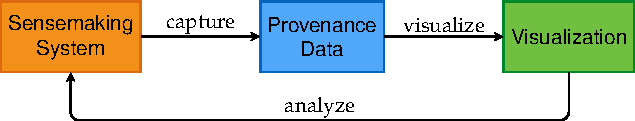
\includegraphics{workflow}
	\caption{A pipeline of supporting sensemaking through analytic provenance. During the process in which a user solves a sensemaking task using a visualization tool, their interactions and discoveries -- we refer to both of them as \emph{provenance data} -- are captured and visualized to provide support back to the sensemaking process.}
	\label{fig:workflow}
\end{figure}

\section{Research Problem and Approach}

\subsection{Problem}
In this thesis, we focus on the \textbf{visualization} part of that process:
\begin{center}
	\strong{How to design interactive visualizations of provenance data \\to support sensemaking?}
\end{center}

%Pirolli and Card~\cite{Pirolli2005} describe sensemaking as a process consisting of two loops: the \emph{foraging loop}, which involves searching, extracting and organizing information; and the \emph{sensemaking loop}, which involves building schemas, generating and testing hypotheses, and presenting the outcome. Schematization plays an important role in this model: connecting the foraging loop and the sensemaking loop. It is a crucial step in converting raw evidence to rational explanations. Pirolli and Card suggest that the schematization process should be supported by a computer-based tool that organizes raw evidence into small-scale stories about typical topics or in answer to typical questions (e.g., who, what, when, where, why, how). This suggestion is aligned with a recent empirical study by Kang, Görg and John Stasko~\cite{Kang2011}. It shows that all of the participants who performed the sensemaking task well spent considerable time and effort in \emph{organizing their collected information}. Their organizational schemes were flexible: a \emph{timeline} of related events, a \emph{map} connecting locations that a person has been to, and a \emph{diagram} showing relationships among suspicious targets.

%One approach to provide such support is through \textbf{analytic provenance} -- an area of research focusing on understanding a user's reasoning process through the study of their interactions with a visualization tool~\cite{North2011}. More specifically, during the process in which a user solves a sensemaking task using a visualization tool, their interactions and discoveries -- we refer to both of them as \emph{provenance data} -- are captured and visualized to provide support back to the sensemaking process itself as summarized in Figure~\ref{fig:workflow}. 



%The research is driven by enabling users to discover the answers to the aforementioned questions (who, what, when, where, why, how) of the captured provenance data.
%\begin{enumerate}
%	\item \strong{when?} this is to help users to analyze the \textbf{temporal} relationship of their provenance data. Current timeline visualization has these limitations
%	\begin{itemize}
%		\item no or very simple layout which is cluttered and space-inefficient
%		\item designed for presenting a known story rather than interactively constructing a hidden one
%	\end{itemize} 
%	\item \strong{who/what?} grouping information related to a person or a topic together allows users to have a better understanding of their provenance data. It is more useful if such \textbf{thematic} information can be visualized together with the temporal information. Currently, this is still an open challenge. These three principles of Gestalt's laws of grouping are typically employed to visualize set relations on a timeline:
%	\begin{itemize}
%		\item similarity: use colors or shapes to indicate sets -- not powerful 
%		\item proximity: not space-efficient
%		\item uniform connectedness: cluttered
%	\end{itemize} 
%	\item \strong{why?} discover and visualize \textbf{semantic/causal} relationships of user's provenance data is a step towards answering this question. After a long period of working on the sensemaking task, the user may get lost. At a low level, they may fail to find the information they discovered before. At a higher level, they may not know where they are in the context of the overall task, and may not know where to continue. Existing visualizations do not fully support users to overcome this \emph{disorientation} problem.
%\end{enumerate}
%
%We choose not to address the \textbf{where} question because spatial information is not always available and relevant to the task. If locations are named, we can consider them as \emph{themes} and use the methods for \textbf{who/what} questions to analyze them. We do not address the \textbf{how} question; however, combining the answers to \textbf{when} and \textbf{who/what} questions may help improve understanding about it.

%We take a user-centered design approach in developing the solutions to the three aforementioned questions. For each question, we elicit the design requirements either by conducting a user study or drawing from the literature. Visual encoding and interaction are designed to meet those requirements and are implemented into a working prototype. Finally, an empirical study is conducted to validate if the tool supports users as intended.  
%
%The analytic provenance approach that we take is general; however, we need to choose specific domains/tasks to demonstrate its application. Sensemaking does not only happen when using a visualization system to solve a ``serious'' intelligence analysis task. Actually, it often happens in our life such as when using a web browser to find information to select the most suitable smartwatch to buy. Therefore, to demonstrate the wide application of our visualization techniques, we target both intelligence analysis tasks using a visualization system and everyday sensemaking tasks using a web browser.

We elaborate the research question by seeking answers to the three practical questions what -- why -- how. This general approach has been used by Aigner~et~al.~\cite{Aigner2011} in their analysis of visualization techniques for time-oriented data and by Brehmer and Munzner~\cite{Brehmer2013} in their characterization of visualization tasks.

%\textch{what} -- \textcm{why} -- \textcb{how}. 

% Explain why this approach first then give sucessful examaples.

\begin{enumerate}
	\item What is presented?
	
	Using the taxonomy of dataset types by Munzner~\cite{Munzner2014}, provenance data can be classified as a \emph{table}, where each row represents an item of data and each column describes an attribute of the dataset. One essential attribute of provenance data is \emph{time} providing when a data item is collected. Categorical information may be added to help make sense of more complex relationship.
	
	The user may also provide additional information to the raw collected data to indicate relationships between data items. This transforms the tabular dataset to a \emph{network} dataset.
	
	\item Why is it presented?
	
	The characteristics of provenance data suggests the tasks it can provide support to users. First, the inherently temporal aspect of provenance data provides an opportunity to allow users to identify temporal patterns and relationships of the sensemaking task. More challengingly, can provenance data help user identify rational relationships of sensemaking?
	
	\item How is it presented?
	
	This depends on the pair data -- task at hand [probably don't need this ``how'']
\end{enumerate}

%Two types of provenance data:
%\begin{itemize}
%	\item user thinking: typically from user notes, high user effort, rich semantics 
%	\item user interaction: automatic capture, no user effort, poor semantics
%\end{itemize}
%
%Two types of relationship in the sensemaking process that provenance data may help to reveal:
%\begin{itemize}
%	\item temporal: understand the process ('how')
%	\item logical: understand the rationale ('why')
%\end{itemize}

\subsection{Approach}

We break down the research problem to the following research questions based on the type of provenance data will be used and the task it aims to support.

\begin{enumerate}
	\item How to design interactive visualization of time-oriented provenance data enabling users to explore temporal relationship of sensemaking?
	
	\item How to design interactive visualization that can utilize both temporal and thematic provenance data to reveal complex temporal relationship of sensemaking?	
	
	\item How to design interactive visualization that can exploit time-oriented provenance data enabling users to explore rational relationship of sensemaking?
	
	\item How to design interactive visualization that can utilize both temporal and relational provenance data enabling users to explore and express complex rational relationship of sensemaking?				
\end{enumerate}

\begin{figure}[!htb]
	\centering
	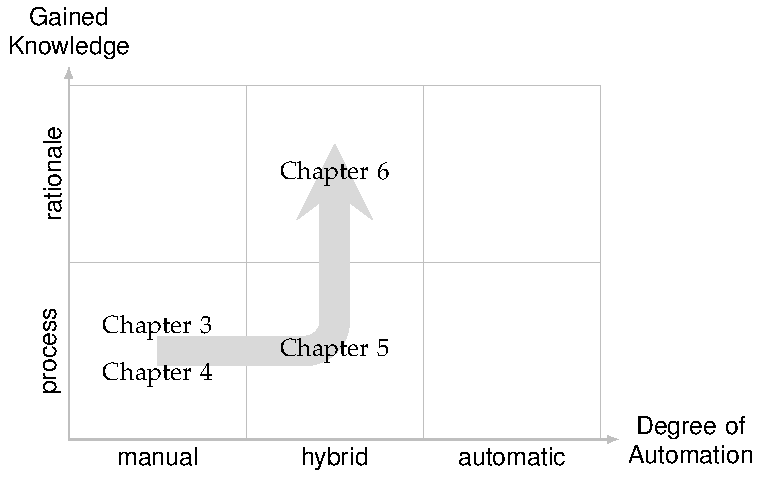
\includegraphics{work}
	\caption{Research problem split by data and task. The horizontal axis represents different tasks and the vertical axis represents the complexity involved in the  task. The cells show the characteristics of data will be used to support the task.}
	\label{fig:work}
\end{figure}


\begin{enumerate}
	\item time $\rightarrow$ temporal relationship
	\item time + theme $\rightarrow$ complex temporal relationship
	\item time $\rightarrow$ rational relationship
	\item time + relation $\rightarrow$ complex rational relationship
\end{enumerate}

Two domains to demonstrate:
\begin{itemize}
	\item intelligence analysis: rigorous sensemaking problems
	\item everyday sensemaking with web browser: popular, high demands
\end{itemize}

We take a user-centered design approach in seeking solutions to all the research questions. For each question, we elicit the design requirements either by conducting a user study and/or drawing from the literature. Visual encoding and interaction are designed to meet those requirements, and the designs are implemented into a working prototype. Finally, an empirical study is conducted to explore how the tool is used by targeted users and whether it supports users as intended. 

\section{Thesis Contributions}
%Chapter 2 provides an overview of sensemaking, visualization and analytic provenance.
%
%Chapter 3 reviews related work of visualizing provenance data to support sensemaking.
%
%Chapter 4 presents a compact yet aesthetically pleasing timeline visualization technique that enables users to interactively construct a temporal schema from provenance data.
%
%Chapter 5 extends Chapter 4 to present a timeline visualization technique that can effectively show both temporal and set information of provenance data. This technique can also be used for more general data.
%
%Chapter 6 discusses the requirements, design, implementation and evaluation of a visualization system that enables users to have an overview of their sensemaking process, to organize their provenance data in such a way that aids their understanding about the task, and to communicate their findings at different levels of granularity.
%
%Chapter 7 describes a general approach that combines analytic provenance and visualization to shorten the transcription and coding steps in qualitative data analysis, and a tool to demonstrate its application.
%
%Finally, Chapter 8 concludes the thesis with a discussion on its contributions and future research directions triggered from this work.

%How to design interactive visualization of time-oriented provenance data to support users in exploring temporal relationships in a dynamic and iterative sensemaking process?
%
%How to design interactive visualization that can utilize both temporal and thematic provenance data to reveal complex temporal relationship of sensemaking?
%
%How to design interactive visualization that can exploit time-oriented provenance data and enable users to explore rational relationship of sensemaking?
%
%How to design interactive visualization that can utilize both temporal and relational provenance data and enable users to integrate their input to explore and express complex rational relationship of sensemaking?



Toward the overall goal of supporting users in their sensemaking processes using provenance data, this thesis contributes:
\begin{itemize}
	\item A timeline visualization technique -- SchemaLine -- that enables users to examine information in chronological order, identify temporal patterns and construct narratives from relevant user annotations. SchemaLine produces a compact but aesthetically pleasing layout and a set of fluid interactions allowing users to perform various sensemaking activities described in the Data--Frame model~\cite{Klein2003}.
	
	\item A timeline visualization technique -- TimeSets -- that enables users to explore complex temporal relationship by effectively representing both temporal and thematic provenance data. TimeSets visually groups data items that share the same theme but still preserves their temporal order. It colors the backgrounds of the entire themes to distinguish them and uses colored gradient backgrounds for the intersections among those themes. It also adjusts the level of details of each data item dynamically to accommodate more items within a given display estate. 
	
	\item Qualitative research methods are often used in understanding rational relationship of sensemaking. This is a manual and time-consuming process: researchers collect observation data, transcribe screen capture videos and think-aloud recordings, identify recurring patterns, and eventually abstract the sensemaking process into a general model. We contribute a visual sensemaking tool -- SensePath -- that offers an alternative and possibly faster approach in performing transcription and coding. In stead of having to transcribe the video, SensePath automatically captures and detects participant's sensemaking actions, and provides multi-linked visualizations to support further analysis. It visualizes provenance data in a timeline that enables researchers to quickly gain an overview of the sensemaking process and identify recurring sensemaking patterns. It also links with a screen capture video to allow researchers to examine  additional context when necessary. Finally, to enable researchers to continue working on later stages of analysis using their normal workflow, SensePath exports its coded transcript in a common format that can be used by other popular qualitative data analysis software packages.	
	
	\item A visual sensemaking tool -- SenseMap -- that enables users to explore and express complex rational relationship of sensemaking. It automatically captures and detects sensemaking actions and relationships between these actions before visualizing both of them in a branching history tree. This allows users to examine the rational relationship between the actions they performed and potentially helps them remind of what have been done earlier. SenseMap offers users to assign additional meaning to the automatically collected data by spatially grouping actions or adding rational links between them, in order to help explain complex relationship. Finally, SenseMap allow users to communicate their analysis results at different levels of granularity including a big picture of user-organized findings, a more detailed analysis process and raw provenance data captured.
\end{itemize}

%mention the papers and co-authors' contributions here
%mention also old SenseMap paper, Rick paper, research agenda?
%list of publication in a separate page

\section{Thesis Outline} 


%\begin{figure}[!htb]
%	\centering
%	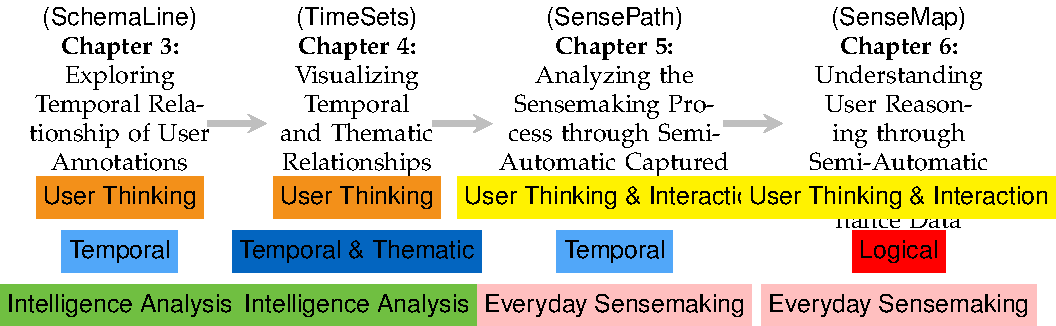
\includegraphics[width=\linewidth]{story}
%	\caption{Summary of upcoming chapters.}
%	\label{fig:story}
%\end{figure}

%\begin{table}[!htb]
%	\centering
%	\sffamily\small
%	\caption{Summary of upcoming chapters.}
%	\label{table:dataset}
%	\begin{tabularx}{\columnwidth}{YL{.1\columnwidth}L{.15\columnwidth}L{.16\columnwidth}}
%		\toprule
%		\textbf{Chapter} & \textbf{Capture} & \textbf{Relationship} & \textbf{Domain} \\ 
%		\midrule
%		\textbf{Chapter 3:} Exploring Temporal Relationship through User Annotations & Manual & Temporal & Intelligence Analysis \\ \addlinespace
%		\textbf{Chapter 4:} Visualizing Temporal and Thematic Relationships & Manual & Temporal \& Thematic & Intelligence Analysis \\ \addlinespace
%		\textbf{Chapter 5:} Analyzing the Sensemaking Process through Semi-Automatic Provenance Capture & Semi-Automatic & Temporal & Everyday Sensemaking \\ \addlinespace
%		\textbf{Chapter 6:}  Understanding High-level Reasoning through Semi-Automatic Provenance Capture & Semi-Automatic & Logical & Everyday Sensemaking \\ 
%		\bottomrule
%	\end{tabularx} 
%\end{table}


%Chapter 2 provides an overview of sensemaking, visualization and analytic provenance.
%
%Chapter 3 reviews related work of visualizing provenance data to support sensemaking.
%
%Chapter 4 presents the design, layout and evaluation of a timeline visualization technique that is designed to support sensemaking.
%
%Chapter 5 extends the timeline visualization in Chapter 4 to include thematic information.
%
%Chapter 6 discusses the requirements, design, implementation and evaluation of SenseMap -- a browser plugin that enables users to collect, curate and communicate their findings.
%
%Chapter 7 describes 
%
%Finally Chapter 8 concludes the thesis with a discussion on its contributions and future research directions triggered from this work.
